
\documentclass[12pt,oneside]{book}

\usepackage{amsmath} % Advanced math typesetting
\usepackage[utf8]{inputenc} % Unicode support (Umlauts etc.)
\usepackage[explicit]{titlesec}
\usepackage{t1enc}
\usepackage[hungarian]{babel} % Change hyphenation rules
\usepackage{hyperref} % Add a link to your document
\usepackage{graphicx} % Add pictures to your document
\usepackage{listings} % Source code formatting and highlighting
\usepackage[a4paper, top=2.5cm, bottom=2.5cm, left=3.5cm, right=2.5cm]{geometry}
%\usepackage{sidecap}
\usepackage{wrapfig}
\usepackage{enumitem}
\usepackage{parskip}

\usepackage{setspace}
\onehalfspacing

%\linespread{1.3}

\begin{document}

% Belső fedőlap

\begin{titlepage}

\noindent
\begin{minipage}{4cm}
    
\includegraphics[width=3cm]{images/cimer_nagy_szines.png}
\end{minipage}
\hfill
\begin{minipage}[c]{8cm}
Eötvös Loránd Tudományegyetem\\
Informatikai Kar\\
Algoritmusok és Alkalmazásaik Tanszék
\end{minipage}

\vspace{5cm}

\begin{center}
\huge
Fizikai alapú 3D megjelenítés valósidőben
\end{center}

\vspace{4cm}

\noindent
\begin{minipage}[t]{7cm}
\flushleft
Valasek Gábor\\
tanársegéd
\end{minipage}
\hfill
\begin{minipage}[t]{5.2cm}
%\flushright
Bölöny Zsolt\\
programtervező informatikus
\end{minipage}

\vspace{1cm}

\noindent
\begin{minipage}[t]{7cm}
\flushleft
Dr. Magdics Milán\\
adjunktus
\end{minipage}

\begin{center}
Budapest, 2016
\end{center}

\end{titlepage}

% Tartalomjegyzék

\tableofcontents

% Bevezetés

\chapter{Bevezetés}

A számítógépes grafikával foglalkozó kutatókat, fejlesztőket napjainkban is foglalkoztatja a kérdés, hogyan lehet a számítógép segítségével minél életszerűbb, \textit{fotorealisztikus} megjelenítést létrehozni. A különféle sugárkövetéses technikákkal már régóta képesek vagyunk rendkívül élethű képek létrehozására, de ezek a módszerek nem minden esetben jelentenek megoldást, hiszen a rendelkezésre álló számítási kapacitástól függően a létrehozás folyamata akár napokig is eltarthat. Míg egy animációs film esetében van lehetőség ezt kivárni, addig a valós idejű megjelenítésben nem áll rendelkezésre ennyi idő: a szinte folyton változó, interaktív 3D-s környezetet a másodperc törtrésze alatt kell a képernyőre vetítenünk.

A grafikus kártyák teljesítménye a megjelenésük óta folyamatosan, gyors ütemben fejlődik. Évről évre újabb és újabb technikák jelennek meg, amelyek igyekeznek kihasználni ezt a folyton növekvő teljesítményt annak érdekében, hogy minél látványosabb, minél valószerűbb legyen a virtuálisan létrehozott 3D-s tartalmak megjelenítése. A fizikai alapú megjelenítés is csupán egy, bár annál jelentősebb módszer ezek közül: nem csak a korábban mindenki által használt Blinn-Phong közelítést cseréli le egy, az anyagok valós, fizikai tulajdonságait figyelembe vevő új módszerre, hanem a megjelenítés bemeneteként szolgáló anyagmodellek előállításának folyamatát is átformálja.

A fizikai alapú megjelenítés (hivatalosan \textit{physically based rendering}, a továbbiakban PBR) legfontosabb tulajdonsága az, hogy az anyagok ill. fények mérhető fizikai tulajdonságait veszi alapul, és az adott pontban a kamera által érzékelt fény színét és intenzitását igyekszik ismert, valós fizikai képletek közelítéseinek segítségével meghatározni. Habár a PBR alapelvei és összefüggései létrejötte óta változatlanok, a felhasznált különféle egyenletek minél pontosabb és mindeközben minél kevésbé számításigényes közelítése a mai napig aktív kutatási terület.

A fizikai alapú megjelenítés előnyeinek bemutatására egy egyszerű modellek betöltésére képes megjelenítőt hoztam létre, amelynek segítségével akár egy témában kevésbé járatos felhasználó számára is láthatóvá válnak a módszer előnyei. A program megalkotása komoly kihívást jelentett, hiszen nem csak a CPU-t, hanem a GPU-t is programoznom kellett árnyalók (\textit{shaderek}) segítségével. A felhasznált technológia újdonsága, az implementáció komplexitása és a várható látványos végeredmény miatt esett választásom erre a feladatra.


\chapter{Felhasználói dokumentáció}

\section{A program üzembe helyezése}



\section{A felhasználói felület áttekintése}

% ábra


\chapter{Fejlesztői dokumentáció}

\section{Elméleti alapozás}

Mielőtt a konkrét implementáció ismertetésére térnénk, fontosnak tartok néhány alapvető matematikai és fizikai fogalmat tisztázni, hiszen a fizikai megjelenítés (igen komoly matematikai hátterű) elmélete ezekre épül, és a későbbiekben gyakran találkozhatunk velük.

felületi integrál, kapcsolódó fogalmak

radiometriai fogalmak

\subsection{Bevezetés}

Tetszőleges térbeli jelenet leképezéséhez alapvetően három dolog szükséges:

\begin{itemize}[noitemsep]
\item a jelenet geometriájának leírása,
\item egy pont a térben, ahonnan "nézzük" a jelenetet, továbbá
\item legalább egy fényforrás, ill. annak pozíciója.
\end{itemize}

Valósidejű grafikában a geometriák leírásához háromszöghálókat használunk, mivel a GPU-k térbeli háromszögeken dolgoznak. Domború felületek leírásához ezen háromszögháló felbontását növeljük addig, amíg a végeredmény szempontjából elfogadható közelítést kapunk. Ezt a folyamatot tesszelációnak hívjuk. Az "elfogadhatóság" teljesen szubjektív tulajdonság, így az egyetlen objektív behatároló tényező a grafikus hardver teljesítménye, amelynek folyamatos fejlődése ezen a téren remekül illusztrálható.

\begin{figure}[!ht]
    \centering
    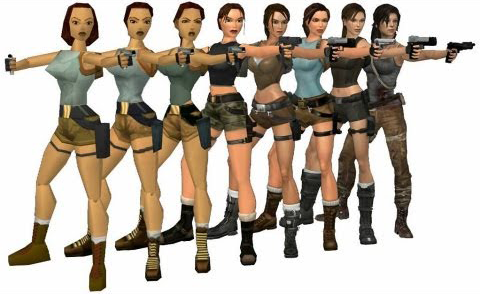
\includegraphics[width=0.5\textwidth]{images/tomb_raider_evolution.png}
    \caption{A Tomb Raider játéksorozat főszereplőjének evolúciója (1996-2013)}
\end{figure}

Önmagukban a háromszögeket meghatározó térbeli pozíciók még nem elégségesek. Ismernünk kell a felület tetszőleges pontjának irányultságát, amelyet egy, a felületből "kifelé" álló, egység hosszúságú vektorral írunk le és felületi normálvektornak hívunk. Jelölése: \(\mathbf{n}\).
%TODO: ezt inkább a gyakorlati részhez, a vertex definíciójával együtt?
Ezeket legegyszerűbben a háromszögeket alkotó pontokkal együtt tárolhatjuk, majd ezeket menet közben interpolálva kaphatjuk meg a háromszög által meghatározott felület tetszőleges pontján vett normálvektort.

\subsection{Az árnyalási egyenlet}

A számítógépes grafika egyik alaptételének tekinthető árnyalási egyenletet (\textit{rendering equation}) David Immel et al.~\cite{immel1986radiosity} és James Kajiya~\cite{kajiya1986rendering} írta le 1986-ban. Az egyenlet segítségével meghatározható a felület egy adott pontját elhagyó sugárzás a felület által kibocsátott ill. visszavert sugárzás összegének geometriai optika alapú közelítésével:

\[
L_0(\mathbf{x},\mathbf{v}) = L_e(\mathbf{x},\mathbf{v}) + \int_\Omega f_r(\mathbf{x},\mathbf{l},\mathbf{v}) L_i(\mathbf{x},\mathbf{l}) (-\mathbf{l} \cdot \mathbf{n})\,\mathrm{d}\mathbf{l}
\]

\noindent
ahol a paraméterek:

\begin{itemize}[noitemsep]
\item \(\mathbf{x}\) a felület egy pontja,
\item \(\mathbf{v}\) a felület egy pontjából a nézeti pozícióba mutató normálvektor (nézeti vektor),
\item \(\mathbf{n}\) a korábban bevezetett felületi normálvektor,
\item \(\mathbf{l}\) pedig a felület egy pontjából a fényforrás felé mutató normálvektor.
\end{itemize}

\noindent
\textit{Megjegyzés: az eredeti egyenlet figyelembe veszi még az időt és a fény hullámhosszát is. Az egyenlet paraméterei az idő előrehaladtával ritkán változnak, és ebben az esetben is előre kiszámolhatóak, ezért gyakorlati alkalmazás esetén az időt állandónak tekinthetjük, amely így kiesik az egyenletből. Mivel számítógépes grafikánál RGB színtérben dolgozunk, és ennek 3 összetevőjét külön-külön számolhatjuk, így a hullámhossz paraméter is elhagyható. A továbbiakban ezért fény alatt a fény színét és erősségét értjük.}

A könnyebb érthetőség kedvéért bontsuk részekre az egyenletet. A bal oldalon szereplő \(L_0\) az eredmény: a felület egy pontjából érkező fényt határozza meg a nézeti vektor függvényében, később ez lesz a ténylegesen megjelenített színérték. A jobb oldal első tagja, \(L_e\) a felület egy pontjából kisugárzott fényt adja meg. Ez az érték a gyakorlatban jellemzően 0, mert kevés emisszív anyag létezik, de pl. a fényforrások megjelenítéséhez szükség van rá. A következő tag az integrál, amelyben az \(\Omega\) a felületi normálvektor körül vett félgömböt jelenti, ami az összes lehetséges \(\mathbf{l}\) vektort tartalmazza, amelyen integrálni kell a tartalmazott függvényeket. Mint később látni fogjuk, az integrálás lesz az egyik sarkalatos pontja az egyenlet gyakorlati alkalmazásának, ugyanis az integrálnak nem minden fényforrás esetén van analitikus megoldása - ilyenkor közelítést fogunk alkalmazni. \(f_r\) az ún. kétirányú visszaverődési eloszlásfüggvény (bi-directional reflection distribution function, röviden BRDF), amely a nézeti irányba visszavert fény és a fényforrás felől besugárzott fény arányát adja meg. A BRDF nagy előnye, hogy fizikailag mérhető, és az interneten található MERL adatbázis 100 különböző anyag visszaverődési függvényét tartalmazza. Tulajdonságai:

\begin{itemize}[noitemsep]
\item pozitív: \(f_r(\mathbf{x},\mathbf{l},\mathbf{v}) \geq 0\)
\item szimmetrikus: \(f_r(\mathbf{x},\mathbf{l},\mathbf{v}) = f_r(\mathbf{x},\mathbf{v},\mathbf{l})\)
\item teljesíti az energiamegmaradás törvényét: \(\int_\Omega f_r(\mathbf{x},\mathbf{l},\mathbf{v}) (-\mathbf{l} \cdot \mathbf{n})\,\mathrm{d}\mathbf{l} \leq 1\)
\end{itemize}

Az \(L_i\) függvény a felület adott pontjára \(-\mathbf{l}\) irányból beérkező fényt adja meg. Fontos megjegyezni, hogy ez a fény nem csak direkt, hanem indirekt forrásból is érkezhet (pl. már valahol tükröződött fény, ld. globális/kép alapú megvilágítás). Az utolsó tag, \(-\mathbf{l} \cdot \mathbf{n}\) a beérkező fény iránya és a felületi normálvektor által bezárt szög koszinusza alapján csökkenti a kisugárzott fény erősségét.

\subsection{Fizikai alapú megjelenítés}

\section{Gyakorlati megvalósítás}

Egy háromdimenziós megjelenítő fejlesztésekor mind programozási nyelv, mind megjelenítő API szempontjából több választási lehetőség áll előttünk. Valósidejű megjelenítőről lévén szó azonban nagyon fontos, hogy a választott programozási környezet járulékos lassító tényezői (pl. menedzselt nyelvek - Java, C\#, stb. - esetén a futtatókörnyezet, ill. szemétgyűjtő futási sebességre és felhasznált memóriára vonatkozó negatív hatása) minél kevésbé befolyásolja a program futását. Ezért - követve az iparág nagy szereplőit - választásom a C++ programozási nyelvre esett. A C++ fordított nyelv, azaz forráskódunkból a processzor által közvetlenül végrehajtható, a fordító által erősen optimalizált gépi kód készül. Ennek egyik hátránya, hogy processzor architektúrához és operációs rendszerhez kötődő futtatható állományt kapunk, azaz minden kívánt platformra külön le kell fordítsuk forráskódunkat - ellentétben pl. a Java-val, amely platformfüggetlen bájtkódot állít elő, és azt a gépre előre telepített, platformspecifikus futtatókörnyezet hajtja végre. Előnye viszont, hogy minden platformra külön optimalizált futtathatót készíthetünk, ami valósidejű megjelenítésnél a futási sebesség szempontjából fontos lehet. A C++ eléggé alacsonyszintű ahhoz, hogy minden teljesítmény szempontjából számító befolyásoló tényezőt (pl. memóriafoglalás, annak pontos ideje és mérete) a kezünkben tarthassunk, de közben eléggé magasszintű ahhoz, hogy az objektum-orientált programozást lehetővé tevő nyelvi eszközei és standard könyvtára (\textit{standard template library, STL}) segítségével hatékonyan írhassunk benne összetett programokat. A megjelenítő fejlesztése során igyekeztem minél jobban igénybe venni az új C++ szabványok (C++11, C++14) által bevezetett szintaktikai és STL-t érintő újdonságokat (okos mutatók, új tömb tároló, automatikus típuslevezetés, stb.), illetve a "modern C++" meghatározó eszközeit (kivételkezelés, RAII), amelyek segítségével egy átlátható, könnyedén bővíthető, robosztus kódbázis született.

Az asztali számítógépeken a két legelterjedtebb grafikus API a DirectX és az OpenGL. Okostelefonokon az OpenGL speciális, kisebb tudású, áramvonalasított változata, az OpenGL ES az egyeduralkodó API. A konzolokon jellemzően erősen specializált alacsonyszintű felületek állnak rendelkezésre, amelyek elérése külön feltételekhez kötött, így ezekről kevés információnk áll rendelkezésre. A két rivális asztali API közül azért OpenGL-re esett a választásom, mert volt már vele tapasztalatom, és mert keresztplatformos, míg a DirectX csak Microsoft Windows rendszeren érhető el.

Ezen szakdolgozat írásának idején jelentek meg vulkan, stb.

\subsection{A felhasznált nyílt forráskódú könyvtárak bemutatása}

Munkám során a fejlesztést megkönnyítendő, és a programozás egyik alapvető tételét, az újrafelhasználást figyelembe véve a fizikai megjelenítéshez szorosan nem kapcsolódó részeket nyílt forráskódú könyvtárak segítségével valósítottam meg. A megjelenítő ablakának ill. az OpenGL környezet létrehozását, továbbá az ehhez kapcsolódó eseménykezelést (egérmozgás, billentyűzet kezelés, ablakesemények) a C-ben írt, keresztplatformos GLFW könyvtár végzi. Ahhoz, hogy az OpenGL bővítményeit használni tudjam, a Python alapú GLAD OpenGL függvénymutató-betöltővel generáltam C forrásfájlt, amelyben a legújabb, 4.5-ös OpenGL verzióig az összes függvénymutató, ill. az ezeket inicializáló mechanizmus megtalálható. Grafikus alkalmazásoknál, kiváltképp három dimenzióban elkerülhetetlen a lineáris algebra használata. Ehhez a népszerű GLM fejléc alapú C++ sablonkönyvtárat választottam, amely az OpenGL árnyalónyelve, a GLSL mintájára készült, és a legfontosabb lineáris algebrai konstrukciók (egész és lebegőpontos vektorok, mátrixok, kvaterniók) mellett többek közt az ezek között definiált műveletek megvalósítását és sok hasznos segédfüggvényt (pl. vetítési, nézeti mátrix létrehozása) is tartalmaz. A megjelenítő elsődleges bemenetét képező 3D-s Wavefront OBJ formátumú modellek betöltését a tinyobjloader C++ könyvtár végzi, amely a hozzájuk csatolt anyagtulajdonság-leíró fájlokat (.mtl kiterjesztéssel) is feldolgozza. A felhasználói felület megjelenítéséért és kezeléséért az OpenGL alapú NanoGUI könyvtár felel, amely a NanoVG (szintén OpenGL-alapú) közvetlen módú vektorgrafikus rajzoló könyvtárra épül. Ezen könyvtárak mindegyike nyílt forráskódú és folyamatos fejlesztés alatt áll, így probléma esetén a szükséges módosításokat végre tudtam hajtani rajtuk, ami - mindamellett, hogy segítségükkel a fizikai megjelenítés konkrét implementációjára koncentrálhattam - nagy segítséget jelentett a fejlesztés során.

\subsection{A megjelenítő felépítése}

Ábra

Ugyan az OpenGL egy meglehetősen magas szintű grafikus programozási felület, a kódismétlés elkerülése és az átláthatóság könnyítése érdekében több egyszerű burkoló objektumot is létrehoztam a leggyakrabban használt OpenGL objektumok köré.

\subsection{Nagy dinamikatartományú megjelenítés}

A jelenleg elterjedt kijelzők túlnyomó többsége 24 bites RGB bemenet alapján dolgozik. Ez azt jelenti, hogy a képernyőn látható színek vörös, zöld és kék komponensekből állnak, ahol minden komponensre \(2^8\) bit jut, azaz 256 különböző értéket vehetnek fel. Elméletben tehát \(3 \cdot 2^8\), azaz körülbelül 16,7 millió különböző színt tudunk megjeleníteni. A valóságban ténylegesen megjelenített színmennyiség a kijelzők különböző fizikai paramétereitől függően változik, de az emberi szem csupán körülbelül 10 millió színt képes megkülönböztetni egymástól~\cite{judd1975color}, így ebben a tekintetben a technológia az emberi érzékelés előtt áll.

Van azonban egy másik nagyon fontos, megjelenítőt és érzékelőt egyaránt jellemző tulajdonság, a kontrasztarány, amit a legvilágosabb (fehér) és a legsötétebb (fekete) megjeleníteni/érzékelni képes szín közötti arányként definiálunk. Míg egy modern LCD kijelző a 24 bites színtér által meghatározott 256:1 bemenő kontrasztarányból kb. 1000:1 kimenő arányt tud megjeleníteni, addig az emberi szem különböző fényviszonyokhoz való rendkívül jó alkalmazkodóképességének köszönhetően ennél jóval nagyobb, kb. 1000:1 - 15000:1 kontrasztarány érzékelésére is képes. (hivatkozás?)

A nagy dinamikatartomány (\textit{high-dynamic-range, HDR}) fogalma először a fényképészet területén jelent meg. A probléma az volt - illetve mind a mai napig az, hogy a fényképezőgépek felépítéséből adódóan egyetlen expozícióval nem lehet olyan képet készíteni, amely visszaadja az emberi szem által érzékelhető dinamikatartományt. A fényképészek ezt úgy oldották meg, hogy az expozíciós időt - és ezzel a bejövő fénymennyiséget - változtatva több képet készítettek ugyanarról a jelenetről, majd egy végső lépésben (színleképezés, \textit{tone mapping}) ezeket egy meghatározott metodika alapján egy képpé kombinálták. A fényképészet a dinamikatartományt ún. expozíciós értékkel (\textit{exposure value, EV}) méri, ahol EV eggyel való növekedése a beérkező fénymennyiség megkétszereződését jelenti.

Ahhoz tehát, hogy az általunk a valóságban érzékelhető fényerősség különbségeket érzékeltetni tudjuk, először is el kell szakadjunk az ebben minket korlátozó 24 bites színtértől. A modern grafikus kártyák már hardveresen támogatják a lebegőpontos (komponensenként 16 vagy 32 bites) puffereket, így ezeket használhatjuk HDR megjelenítésre. A fényképészettel ellentétben továbbra is csak egy leképezési lépésre van szükségünk, amely során egy ilyen lebegőpontos pufferbe számolunk, amelyben a korábbi maximális 255-nél fényerősségtől függően jóval nagyobb értékek is szerepelhetnek. A kijelzők azonban továbbra is a 24 bites, alacsony dinamikatartományú RGB színtérben várják a bemenetet, ezért HDR megjelenítésnél is szükség van egy színleképezési lépésre, amely során egy ún. színleképezési operátor segítségével a pufferben szereplő értékeket ismét "beszorítjuk" a \([0, 1]\) intervallumba. Színleképezés során az alapvető cél az eredeti HDR kép lokális kontrasztarányainak minél jobb megtartása. Több ilyen operátor létezik, az egyik legegyszerűbb ezek közül a Reinhard operátor~\cite{reinhard2002photographic}:

\[
L_{ldr} = { L_{hdr}(x, y) \over 1 + L_{hdr}(x, y) }
\]

ahol \(L_{hdr}(x, y)\) a (kétdimenziós) HDR puffer \((x, y)\) koordinátájában található érték.

Az elkészített megjelenítő három választható színleképezési operátort tartalmaz, amelyek megvalósítása a tone\_map.fs.glsl árnyalóban található. Az első az alapértelmezett Uncharted 2, amelyet készítői "filmszerűnek" hívnak mozi-szerű színvilága miatt. Ezen kívül a fent említett Reinhard, illetve az Unreal Engine 4 alapértelmezett operátora került megvalósítása. Míg az előbbi igen fakó kimenetet ad, addig az utóbbi jelentősen megnöveli a színtelítettséget.

Nagy dinamikatartományú megjelenítéssel tehát jól modellezhetők a való világban tapasztalható fényviszonyok. Ugyanakkor egy új probléma is felmerül, mégpedig a fényviszonyokhoz történő adaptáció. Amikor például egy sötét szobából hirtelen kilépünk egy napsütötte teraszra, a szemünk - bizonyítva rendkívüli alkalmazkodóképességét - alkalmazkodik a hirtelen megváltozott fényerőhöz, pupillánk összeszűkül, hiszen a megnövekedett fénysűrűség miatt elég kisebb területen mintát vennie a színek megállapításához. Ezen effektus megvalósítása szinte kötelező egy HDR megjelenítő esetén, ugyanis hiába használunk nagy dinamikatartományt, enélkül a kevéssé vagy erősen megvilágított jelenetek természetellenesen sötétnek vagy világosnak hatnának.

A megvalósításhoz szükségünk van a jelenet átlagos fénysűrűségére, amely Erik Reinhard módszerével~\cite{reinhard2002photographic} a következőképpen számolható:

\[
L_{avg} = exp\left( { 1 \over N } \displaystyle\sum_{x, y} log(\delta + L_{rel}(x, y)) \right)
\]

ahol

\begin{itemize}[noitemsep]
\item \(N\) a HDR puffer képpontjainak száma,
\item \(\delta\) egy kis érték \(log(0)\) elkerülésére abban az esetben, ha van fekete pixel a pufferben,
\item \(L_{rel}\) pedig a puffer \((x, y)\) pontjában vett relatív fényerősség.
\end{itemize}

Ennek implementációja az average\_luminance.fs.glsl árnyalóban található, lépései a következők: először egy \(64 \times 64\)-es textúrába számoljuk ki a \(log\) értékeit, majd ezt egyszerű átlagszámítással csökkentjük előbb \(16 \times 16\)-os, majd \(4 \times 4\)-es és végül \(1 \times 1\)-es méretűre. Utolsó lépésként ezen az egy értéken az \(exp\)-et elvégezve kapjuk \(L_{avg}\)-t. Az első lépéshez szükségünk van a relatív fényerősségre, amely egy \([0; 1]\) intervallumba eső érték. RGB színtér esetén háromelemű színvektorral dolgozunk, ebből triviálisan átlagot számolva (\( { R + G + B } \over 3 \)) kaphatunk ilyen értéket. Szemünk viszont nem egyformán érzékeli a három alapszínt: az ún. fényerősség függvény (\textit{luminosity function}) alapján a zöld színre sokkal érzékenyebbek vagyunk, mint a vörösre vagy a kékre. Ezt figyelembe véve a fényerősség függvény és az azon alapuló sRGB konverzióból~\cite{stokes2012standard} származó konstans fényerősség vektor segítségével a következőképpen számolhatjuk a relatív fényerősséget:

\[
L_{rel} = [0.2126, 0.7152, 0.0722] \cdot L_{hdr}
\]

Mivel a színleképezés expozíció alapján működik, ezért az átlagos fénysűrűségből ezt valahogyan ki kell számoljuk. A DICE prezentációja~\cite{dice_moving_frostbite_to_pbr} alapján:

\[
EV = log_2\left({ L_{avg} \cdot S } \over K\right)
\]

ahol

\begin{itemize}[noitemsep]
\item \(S\) a kamera ISO értéke,
\item \(K\) pedig egy eszközfüggő kalibrációs állandó.
\end{itemize}

Ebből látható, hogy az expozíciós érték definíciója függ az ISO értéktől. Mivel a mi esetünkben \(EV\)-t fénymennyiség mérésére használjuk, ezért az ISO-t 100-ban rögzítjük, és ezentúl \(EV_{100}\)-ként hivatkozunk rá. A \(K\) állandó értékét az ISO 2720:1974 szabvány 10,6 és 13,4 között javasolja meghatározni. Én - a legtöbb modern 3D megjelenítőhöz hasonlóan - 12,5-nek választottam, így

\[
EV_{100} = log_2\left({ L_{avg} \cdot 100 } \over 12,5\right)
\]

Az expozíció ebből a DICE prezentációja alapján a következőképpen számolható:

\[
exposition = { 1 \over { 1,2 \cdot 2^{EV_{100}} } } = { 1 \over { 9,6 \cdot L_{avg} } }
\]

A színleképezés bemenetét képező \(L_{hdr}\) vektort ezzel az expozícióval megszorozva a fényerő-adaptáció működésbe lép.

A valóban élethű fényerősség adaptációhoz még egy dolog szükséges: a késleltetés. Szemünk ugyanis nem azonnal, hanem a változás mértékével arányosan lassan, fokozatosan alkalmazkodik a megváltozott fényviszonyokhoz. Ehhez el kell tároljuk a legutóbbi képkoca kirajzolása során mért átlagos fénysűrűséget, így a legutóbbi és az éppen kirajzolt állapot között az eltelt idő függvényében lineáris interpolációval kiszámolható az adaptáció aktuális mértéke, ezáltal szemünkhöz hasonlóan lassítva a folyamatot. Ennek implementációja a luminance\_adapter.fs.glsl árnyalóban található.

\subsection{Kép alapú megvilágítás}

\subsection{Pont- és zseblámpa fények}

\section{Tesztelés}

Egy 3D megjelenítő tesztelésénél némileg el kell térnünk a manapság széles körben elterjedt automatikus egységtesztelés módszertanától. Ennek oka az, hogy a megjelenítő által előállított kimenet nem egy könnyen ellenőrizhető, másik helyes kimenettel egy az egyben összehasonlítható eredmény (pl. szöveg), hanem egy kép. Ugyan léteznek módszerek két kép objektív összehasonlítására, ha ilyen módszerhez folyamodunk, felmerül a kérdés, hogy mit tekintünk helyes megoldásnak, \textit{referenciának}? Egy, az iparág által fizikai alapú megjelenítők esetében használt módszer a valósidejű mellé egy ugyanazon bemenetet használó, szintén fizikai alapú de sugárkövetésen alapuló megjelenítőt fejleszteni, amellyel aztán a valósidejű megjelenítéshez használt megoldások, közelítések helyessége ellenőrizhető. Fontos kiemelni, hogy itt sem számítógép általi, automatikus összehasonlításról van szó: azt a kimenetet tekintjük helyesnek, amely "ránézésre" jónak, fizikailag plauzibilisnek tűnik. Mivel egy külön sugárkövetéses megjelenítő fejlesztése csupán a tesztelés céljából bőven túlmutat ezen szakdolgozat keretein, ezért a kimenet tesztelésénél a szememre hagyatkoztam, és referenciának egy neves PBR alapú eszközt, a Marmoset Toolbag 2-t használtam.

\subsection{Alapvető funkciók helyes működésének ellenőrzése}

Mielőtt rátérnénk a kimenet tesztelésére, fontos leellenőriznünk, hogy a felhasználói interakció során a program helyesen működik, véd az alapvető felhasználói hibák ellen, illetve a különböző bemeneteket jól kezeli.

\subsection{A kimenet ellenőrzése}

\bibliography{documentation}{}
\bibliographystyle{plain}

\end{document} 